\documentclass{article}
\usepackage[latin1]{inputenc}
\usepackage{enumerate}
\usepackage{hyperref}
\usepackage{graphics}
\usepackage{graphicx}
\usepackage{caption}
\usepackage{subcaption}
\usepackage{tabularx}
\usepackage{amsmath}
\newcommand{\ket}[1]{\ensuremath{\left|#1\right\rangle}}
\newcommand{\bra}[1]{\ensuremath{\left\langle#1\right|}}
\newcommand{\braket}[2]{\ensuremath{\left\langle #1 \middle| #2 \right\rangle}}
\newcommand{\obar}[1]{\ensuremath{\overline{ #1 }}}
% enumerate is numbered \begin{enumerate}[(I)] is cap roman in parens
% itemize is bulleted \begin{itemize}
% subfigures:
% \begin{subfigure}[b]{0.5\textwidth} \includegraphics{asdf.jpg} \caption{} \label{subfig:asdf} \end{subfigure}
\hypersetup{colorlinks=true, urlcolor=blue, linkcolor=blue, citecolor=red}
\graphicspath{ {C:/Users/Evan/Desktop/} }
\title{Assignment 2: \\ Introduction to \emph{Mathematica}\\
\large \emph{Introduction to Data Analysis for Physics}}
\author{Evan Ott and Will Beason}
\date{Spring 2014}
\setcounter{secnumdepth}{0}
\usepackage[parfill]{parskip}
\begin{document}
\maketitle
\section{Submission Requirements}
Submit the assignment to \href{mailto:data.analysis.physics@gmail.com}{data.analysis.physics@gmail.com} by Wednesday at 5pm. Just submit the \emph{Mathematica}
document you create (typically a .nb file).

\section{Problem 1}
To start, let's make a simple set of data and use some of the stylistic options to make a graph exactly the way we want. Start with
\begin{verbatim}
data = Table[{i, Sin[.1 i]}, {i, 0, 100}]
\end{verbatim}
and create a plot that matches the one in Figure \ref{fig:listplot}. You may find the \texttt{Style} function useful (updated in reading - just above the Practice Problem for Simple Plots).
To create the plot, I had to use \texttt{PlotStyle, PlotRange, AxesLabel, PlotLabel}, and \texttt{AxesStyle}.

\begin{figure}
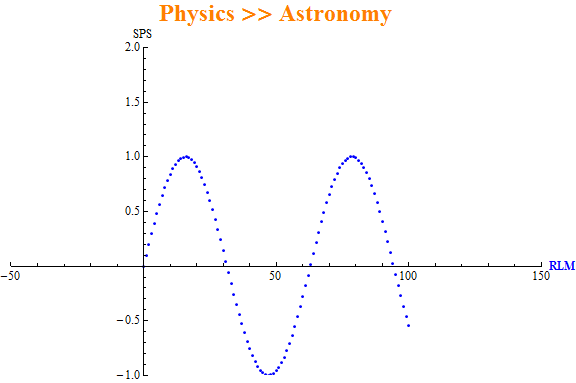
\includegraphics[scale=.6]{physics_astro.png}
\caption{Graph to imitate.}
\label{fig:listplot}
\end{figure}

\section{Problem 2}
Combinatorics are an important facet of probability, which occasionally shows up for physics problems in quantum mechanics / thermodynamics / etc. The \texttt{Binomial[n,m]} function
is the same as $$\left(\begin{array}{c}n\\m\end{array}\right)=\frac{n!}{m!(n-m)!}$$Create a 10x10 matrix with these values, with each row corresponding to a value of $n$ and each
column corresponding to a value of $m$ such that the matrix element $$A_{i,j}=\left(\begin{array}{c}i\\j\end{array}\right)$$ Let's use matrix operations such as indexing and taking the
\texttt{Total} of a list to investigate some properties. In \emph{Mathematica}, having $m>n$ produces 0 - feel free to use this to your advantage or ignore it, depending on how
complicated you want to make things. This problem is meant for you to try many different selections of the data until you find one that's close. If you have to index it
starting on the 3rd row for it to match the expression exactly (for example), that's perfectly acceptable. Any reasonable variation is fine.

\subsection{a}
Find an operation on the matrix that is equivalent to the expression $$\frac{k(k+1)}{2}$$

\subsection{b}
Find an operation on the matrix that is equivalent to the expression $$2^k$$

Note: Don't worry about proving this formally, just try it for a few values and make sure it works.

\section{Problem 3}
With the data below, find a way to plot the relationship between the second grade (taken at the end of the semester for this fictional class) and the first grade multiplied by attendance
(scale attendance from a percent to a fraction while you're at it). For clarity, go ahead and make the points \texttt{Medium} in size, and label the graph appropriately.

\begin{verbatim}
class = {{"Name", "Grade 1", "Grade 2", "Attendance"},
   {"Michael", 95, 93, 20},
   {"George", 95, 87, 90},
   {"Oscar", 50, 78, 60},
   {"Lucille", 100, 0, 10},
   {"Lindsay", 40, 40, 40},
   {"Steve", 0, 0, 100},
   {"Barry", 50, 50, 50},
   {"Ron", 100, 100, 57},
   {"Rita", 10, 20, 97},
   {"Sally", 100, 100, 100},
   {"Maggie", 77, 76, 75}};
\end{verbatim}



\end{document}